\tikzset{%
  % Specifications for style of nodes:
            base/.style = {rectangle, rounded corners, draw=black,
                           minimum width=4cm, minimum height=1cm,
                           text centered, font=\sffamily},
  activityStarts/.style = {base, fill=blue!30},
       startstop/.style = {base, fill=red!30},
    aggclustering/.style = {base, fill=green!30},
         process/.style = {base, minimum width=2.5cm, fill=orange!15,
                           font=\ttfamily},
}
% Drawing part, node distance is 1.5 cm and every node
% is prefilled with white background

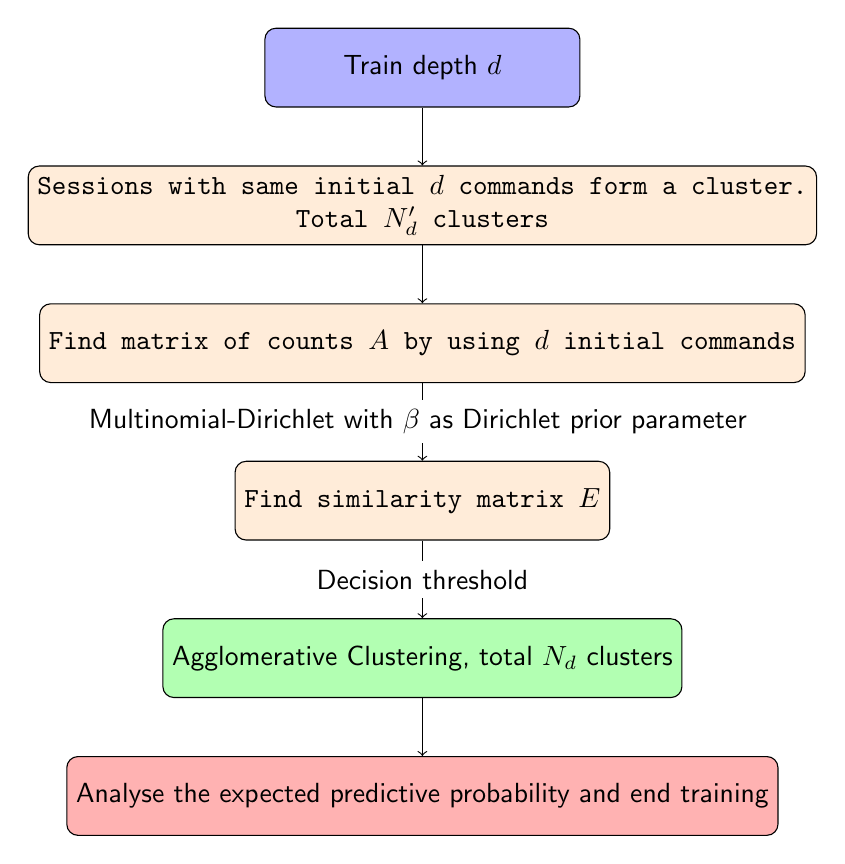
\begin{tikzpicture}[node distance=1.5cm,
    every node/.style={fill=white, font=\sffamily}, align=center]
  % Specification of nodes (position, etc.)
  \node (start)             [activityStarts]              {Train depth \(d\)};

  \node (ncluster)      [process, below of=start, yshift=-0.25cm] 
  {Sessions with same initial \(d\) commands form a cluster.\\Total \(N_d'\) clusters};
  \node (matA)     [process, below of=ncluster, yshift=-0.25cm]          
  {Find matrix of counts $A$ by using \(d\) initial commands};
  \node (matE)      [process, below of=matA, yshift=-0.5cm]   
  {Find similarity matrix $E$};
  \node (aggclustering2)      [aggclustering, yshift=-0.5cm,below of=matE]  
  {Agglomerative Clustering, total \(N_d\) clusters};
  \node (end)      [startstop, yshift=-0.25cm,below of=aggclustering2]  
  {Analyse the expected predictive probability and end training};
  % Specification of lines between nodes specified above
  % with aditional nodes for description 
  \draw[->]      (start) -- (ncluster);
  \draw[->]      (ncluster) -- (matA);
  \draw[->]     (matA) -- node[]{
      Multinomial-Dirichlet with \(\boldsymbol{\beta}\) as Dirichlet prior parameter
  }(matE);
  \draw[->]      (matE) -- node[]{Decision threshold}(aggclustering2);

  \draw[->]      (aggclustering2) -- (end);
\end{tikzpicture}